% Бүлэг 4

\chapter{Хэрэгжилт, туршилт ба үр дүн}
\label{Chapter4}

\section{Хөгжүүлэлтийн орчны бэлтгэл}
Anoce/MFA платформыг Next.js аппликейшн хэлбэрээр хөгжүүлсэн. Хөгжүүлэлтийн үндсэн орчинд Visual Studio Code, Node.js, npm, TypeScript, Next.js, React, Tailwind CSS, CouchDB, Supabase, Git, Chrome browser ашиглав. Төсөл нь root түвшинд Next.js аппликейшн, \path{diplomapaper} хавтас дотор дипломын LaTeX тайлан байрлах бүтэцтэй.

\begin{table}[htbp]
  \centering
  \small
  \begin{tabular}{|L{0.24\textwidth}|L{0.30\textwidth}|L{0.32\textwidth}|}
    \hline
    \textbf{Хэрэгсэл} & \textbf{Үүрэг} & \textbf{Төслийн хэрэглээ} \\ \hline
    Visual Studio Code & Код бичих орчин & Фронтэнд, API, LaTeX тайлан засварлах \\ \hline
    Node.js/npm & JavaScript runtime, package manager & Next.js dev/build/test script ажиллуулах \\ \hline
    Next.js 16 & Full-stack React framework & Public page, admin page, API route \\ \hline
    React 19 & Component-based UI & Карт, форм, overlay, dashboard UI \\ \hline
    TypeScript & Static type checking & Domain type, API data safety \\ \hline
    Tailwind CSS & Styling framework & Responsive layout, visual design \\ \hline
    CouchDB & Document database & Article, designer, collection, asset content store \\ \hline
    Supabase & Auth/user/RAG layer & Authentication, profile role, bookmark, RAG index \\ \hline
    Chrome & Browser testing & Screenshot, responsive UI шалгах \\ \hline
  \end{tabular}
\vspace{0.4em}
  \caption{Хөгжүүлэлтийн орчин}
  \label{tab:development-environment}
\end{table}

\begin{longtable}{|L{0.24\textwidth}|L{0.30\textwidth}|L{0.32\textwidth}|}
  \hline
  \textbf{Хавтас/файл} & \textbf{Үүрэг} & \textbf{Тайлбар} \\ \hline
  \path{app} & Next.js route ба UI & Public page, admin page, API route \\ \hline
  \path{app/components} & Дахин ашиглагдах component & Navbar, hero, cards, search overlay, footer \\ \hline
  \path{app/admin/(protected)} & Admin CMS & Dashboard, articles, collections, designers, assets, users \\ \hline
  \path{app/api/content} & Public content API & Article, collection, designer, search index унших \\ \hline
  \path{app/api/admin/content} & Protected admin API & Content CRUD, asset upload \\ \hline
  \path{lib/couchdb} & CouchDB client/repository & Document conversion, CRUD, attachment \\ \hline
  \path{lib/supabase} & Supabase helper & Auth, role, bookmark, RAG query \\ \hline
  \path{scripts} & Seed/import pipeline & CouchDB болон RAG seed хийх script \\ \hline
  \path{diplomapaper} & Дипломын тайлан & LaTeX source, diagrams, figures, PDF \\ \hline
  \caption{Төслийн файлын бүтэц}
  \label{tab:project-structure-implementation}\\
\end{longtable}

\section{Frontend хэрэгжилт}
Фронтэнд хэрэгжилт нь public уншигчийн интерфэйс болон admin CMS интерфэйс гэсэн хоёр үндсэн хэсэгтэй. Public талд home, archive, designers, editorial, article detail, collection detail, profile, journal, careers, press, global search overlay ажиллана. Admin талд login, dashboard, articles, collections, designers, assets, calendar, users зэрэг хуудас байрлана. Users хуудас нь зөвхөн админд нээлттэй.

\begin{figure}[htbp]
  \centering
  
\includegraphics[width=0.92\textwidth]{Figures/screenshots/homepage_cropped.png}
  \caption[Нүүр хуудасны хэрэгжилт]{Anoce/MFA платформын нүүр хуудасны хэрэгжилт}
  \label{fig:impl-homepage}
\end{figure}

Нүүр хуудас нь brand identity-г хүчтэй харуулах hero section, visual discover section, collection grid, footer гэсэн full-screen snap scroll хэсгүүдтэй. Энэ зохиомж нь fashion magazine-ийн visual-first шинжийг илэрхийлж, хэрэглэгчийг archive болон editorial content руу оруулах entry point болж өгдөг.

\begin{figure}[htbp]
  \centering
  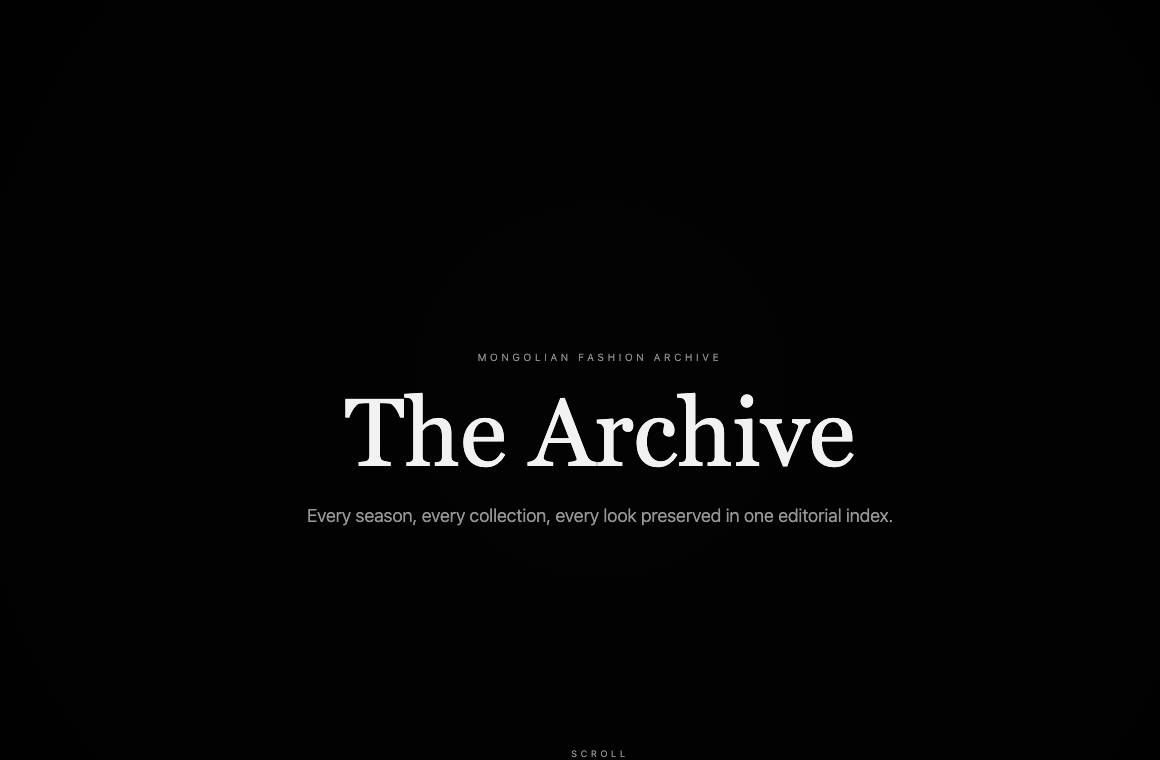
\includegraphics[width=0.92\textwidth]{Figures/screenshots/archive_cropped.png}
  \caption[Archive хуудасны хэрэгжилт]{Archive хуудасны hero ба navigation хэрэгжилт}
  \label{fig:impl-archive}
\end{figure}

Archive page нь collection-уудыг season, year, designer, category, material зэрэг metadata-аар шүүхээр зохиогдсон. Collection detail page-д look зураг, материал, tag, designer relation харуулах боломжтой. Editorial page нь нийтлэлийн featured section, read next, related looks зэрэг сэтгүүлийн унших урсгалтай.

\begin{longtable}{|L{0.24\textwidth}|L{0.32\textwidth}|L{0.30\textwidth}|}
  \hline
  \textbf{Route} & \textbf{Хэрэгжилт} & \textbf{Үр дүн} \\ \hline
  \path{/} & Hero, discover, collections grid, footer & Brand identity болон entry navigation бүрдсэн \\ \hline
  \path{/archive} & Collection grid, filter, archive hero & Collection хайх/шүүх үндсэн орчин бүрдсэн \\ \hline
  \path{/archive/[slug]} & Collection detail, looks, material/tag & Загварын зурагт архивын detail view бүрдсэн \\ \hline
  \path{/designers} & Designer directory, tier filter & Designer profile руу шилжих боломжтой \\ \hline
  \path{/editorial} & Featured story, read next, article list & Сэтгүүлийн нийтлэл унших landing бүрдсэн \\ \hline
  \path{/editorial/[slug]} & Article detail, body, cover image, tags & Нийтлэлийн дэлгэрэнгүй унших боломжтой \\ \hline
  \path{/journal} & Редакцийн тэмдэглэл, чиг хандлагын контент & Монгол тексттэй мэдээллийн хуудас болсон \\ \hline
  \path{/careers} & Ажлын байр, хамтран ажиллах урилга & Монгол хэрэглэгчид ойлгомжтой careers хуудас бүрдсэн \\ \hline
  \path{/press} & Хэвлэл мэдээлэл, brand kit, холбоо барих мэдээлэл & Press мэдээлэл монгол хэлээр бүрдсэн \\ \hline
  \path{/profile} & Profile, bookmark, бүртгэл устгах & Нэвтэрсэн хэрэглэгч өөрийн мэдээллээ удирдана \\ \hline
  \path{/admin/login} & Staff login form & Admin/editor хэрэглэгч нэвтрэх орчин бүрдсэн \\ \hline
  \path{/admin/dashboard} & Content count, recent activity, quick actions & CMS-ийн хяналтын самбар бүрдсэн \\ \hline
  \path{/admin/users} & Invite, role update, team table & Зөвхөн админд нээлттэй хэрэглэгчийн удирдлага бүрдсэн \\ \hline
  \caption{Frontend route хэрэгжилт}
  \label{tab:frontend-implementation}\\
\end{longtable}

\section{Backend хэрэгжилт}
Бэкенд хэрэгжилт нь Next.js API route болон repository layer дээр суурилсан. Public API нь published content унших, admin API нь role шалгасны дараа CRUD хийх, chat API нь AI туслахын context бүрдүүлж хариулт үүсгэх үүрэгтэй. Хэрэглэгч урих, эрх өөрчлөх API нь зөвхөн admin role шалгасны дараа ажиллана.

\begin{longtable}{|L{0.30\textwidth}|L{0.34\textwidth}|L{0.22\textwidth}|}
  \hline
  \textbf{API бүлэг} & \textbf{Хэрэгжилтийн үүрэг} & \textbf{Access} \\ \hline
  \path{/api/content/articles} & Published article list болон detail унших & Public \\ \hline
  \path{/api/content/collections} & Collection list/detail, filter параметр унших & Public \\ \hline
  \path{/api/content/designers} & Designer list/detail унших & Public \\ \hline
  \path{/api/content/search-index} & Search overlay-д хэрэгтэй нэгтгэсэн index үүсгэх & Public \\ \hline
  \path{/api/admin/content/articles} & Article CRUD, draft/review/published status удирдах & Editor/Admin \\ \hline
  \path{/api/admin/content/collections} & Collection CRUD, looks metadata удирдах & Editor/Admin \\ \hline
  \path{/api/admin/content/designers} & Designer CRUD удирдах & Editor/Admin \\ \hline
  \path{/api/admin/content/assets} & Asset upload/list хийх & Editor/Admin \\ \hline
  \path{/api/admin/invite} & Багийн гишүүн урих, viewer/editor/admin эрх оноох & Admin \\ \hline
  \path{/api/admin/users/[id]/role} & Хэрэглэгчийн эрхийг сервер талд шалгаж шинэчлэх & Admin \\ \hline
  \path{/api/profile/delete} & Өөрийн profile, bookmark, auth бүртгэл устгах & Auth \\ \hline
  \path{/api/chat} & Live archive + RAG context ашиглан chatbot хариу үүсгэх & Public/Auth \\ \hline
  \caption{Backend API хэрэгжилт}
  \label{tab:backend-implementation}\\
\end{longtable}

\texttt{lib/couchdb/repository.ts} файл дахь \texttt{ContentRepository} class нь storage detail-ийг API route-уудаас тусгаарладаг. Repository нь \texttt{getArticles}, \texttt{upsertArticle}, \texttt{deleteArticle}, \texttt{getCollections}, \texttt{upsertCollection}, \texttt{getDesigners}, \texttt{createAsset} зэрэг method-оор domain-level үйлдлийг гүйцэтгэнэ. Ингэснээр API route нь raw CouchDB request бичихгүй, харин repository abstraction ашиглана.

\section{Өгөгдлийн сангийн хэрэгжилт}
Өгөгдлийн сангийн хэрэгжилт нь CouchDB болон Supabase гэсэн хоёр давхаргатай. CouchDB-д content document хадгалагдана. Supabase-д authentication, profile role, bookmark/follow, RAG document index хадгалагдана. Энэ бүтэц нь загварын content-ийн уян JSON шинж болон хэрэглэгчийн эрхийн relational/RLS шинжийг тус тусад нь ашиглах боломж өгдөг.

\begin{figure}[htbp]
  \centering
  \resizebox{\textwidth}{!}{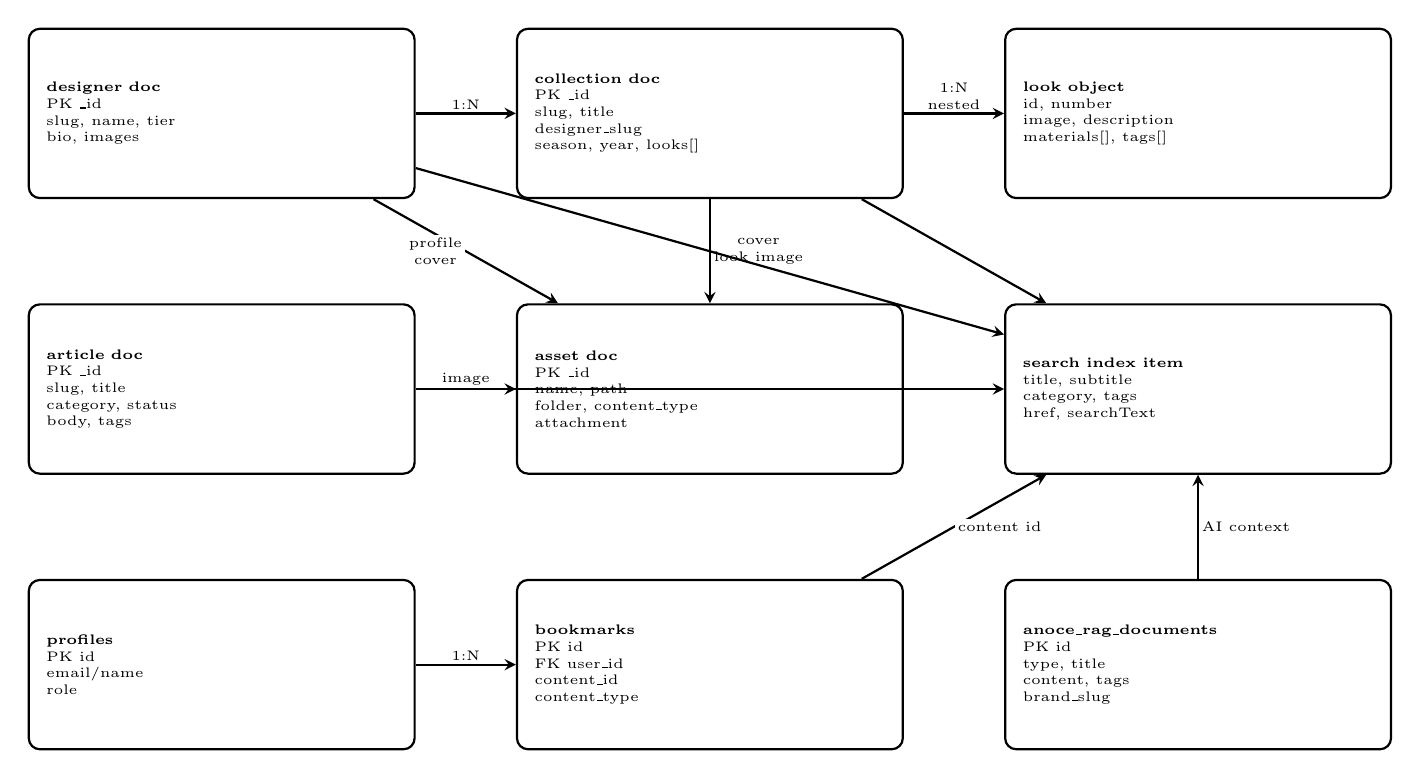
\begin{tikzpicture}[x=1cm,y=1cm,>=stealth,thick]
  \tikzstyle{entity}=[draw, rounded corners=4pt, minimum width=4.9cm, minimum height=2.15cm,
    text width=4.45cm, align=left, font=\tiny]
  \tikzstyle{rel}=[font=\tiny, fill=white, inner sep=1pt, align=center]

  \node[entity] (designer) at (0,6.6) {\textbf{designer doc}\\PK \_id\\slug, name, tier\\bio, images};
  \node[entity] (collection) at (6.2,6.6) {\textbf{collection doc}\\PK \_id\\slug, title\\designer\_slug\\season, year, looks[]};
  \node[entity] (look) at (12.4,6.6) {\textbf{look object}\\id, number\\image, description\\materials[], tags[]};

  \node[entity] (article) at (0,3.1) {\textbf{article doc}\\PK \_id\\slug, title\\category, status\\body, tags};
  \node[entity] (asset) at (6.2,3.1) {\textbf{asset doc}\\PK \_id\\name, path\\folder, content\_type\\attachment};
  \node[entity] (search) at (12.4,3.1) {\textbf{search index item}\\title, subtitle\\category, tags\\href, searchText};

  \node[entity] (profile) at (0,-0.4) {\textbf{profiles}\\PK id\\email/name\\role};
  \node[entity] (bookmark) at (6.2,-0.4) {\textbf{bookmarks}\\PK id\\FK user\_id\\content\_id\\content\_type};
  \node[entity] (rag) at (12.4,-0.4) {\textbf{anoce\_rag\_documents}\\PK id\\type, title\\content, tags\\brand\_slug};

  \draw[->] (designer) -- node[above,rel] {1:N} (collection);
  \draw[->] (collection) -- node[above,rel] {1:N\\nested} (look);
  \draw[->] (article) -- node[above,rel] {image} (asset);
  \draw[->] (collection) -- node[right,rel] {cover\\look image} (asset);
  \draw[->] (designer) -- node[left,rel] {profile\\cover} (asset);
  \draw[->] (designer) -- (search);
  \draw[->] (collection) -- (search);
  \draw[->] (article) -- (search);
  \draw[->] (profile) -- node[above,rel] {1:N} (bookmark);
  \draw[->] (bookmark) -- node[right,rel] {content id} (search);
  \draw[->] (rag) -- node[right,rel] {AI context} (search);
\end{tikzpicture}
}
  \caption[Өгөгдлийн сангийн хэрэгжилтийн бүтэц]{CouchDB document ба Supabase relational layer-ийн бүтэц}
  \label{fig:impl-database-er}
\end{figure}

\begin{longtable}{|L{0.20\textwidth}|L{0.34\textwidth}|L{0.32\textwidth}|}
  \hline
  \textbf{Document} & \textbf{Гол талбар} & \textbf{Хэрэглэх хэсэг} \\ \hline
  \texttt{designer} & slug, name, brand, tier, bio, profile/cover image & Designers page, collection relation, search \\ \hline
  \texttt{collection} & slug, title, designer\_slug, season, year, looks[] & Archive page, collection detail, AI context \\ \hline
  \texttt{article} & slug, title, category, status, body, tags, cover image & Editorial page, admin articles, search \\ \hline
  \texttt{asset} & name, folder, content\_type, size, attachment & Cover/look/profile image serve хийх \\ \hline
  \caption{CouchDB document хэрэгжилт}
  \label{tab:couchdb-doc-implementation}\\
\end{longtable}

Seed pipeline нь demo content-ийг CouchDB руу оруулахад ашиглагдана. \path{scripts/seed-couchdb.ts} нь монгол хэл дээр бэлтгэсэн designer, collection, article өгөгдлийг repository-оор дамжуулан upsert хийдэг. \path{scripts/seed-anoce-rag.ts} нь curated RAG dataset болон нэмэлт archive context-ийг Supabase дахь \path{anoce_rag_documents} хүснэгтэд import хийхээр зохиогдсон. Ингэснээр public UI болон AI туслахын жишээ контент англи placeholder бус, Монгол хэрэглэгчид ойлгомжтой өгөгдөлд тулгуурлана.

\section{Authentication ба authorization хэрэгжилт}
Authentication буюу нэвтрэлт танилт нь хэрэглэгчийг таних, authorization буюу эрхийн шалгалт нь тухайн хэрэглэгч ямар үйлдэл хийх эрхтэйг шалгах үүрэгтэй. Платформд Supabase Auth ашиглан хэрэглэгчийн session авна. Admin route болон admin API-д \texttt{profiles.role} талбараар editor/admin эрх шалгана. Viewer буюу энгийн уншигчид admin CMS-д хандах боломжгүй. Редактор контентын хэсгүүдэд ажиллах боломжтой боловч \path{/admin/users}, \path{/api/admin/invite}, \path{/api/admin/users/[id]/role} зэрэг хэрэглэгчийн эрхтэй холбоотой үйлдэл зөвхөн админд нээлттэй.

\begin{figure}[htbp]
  \centering
  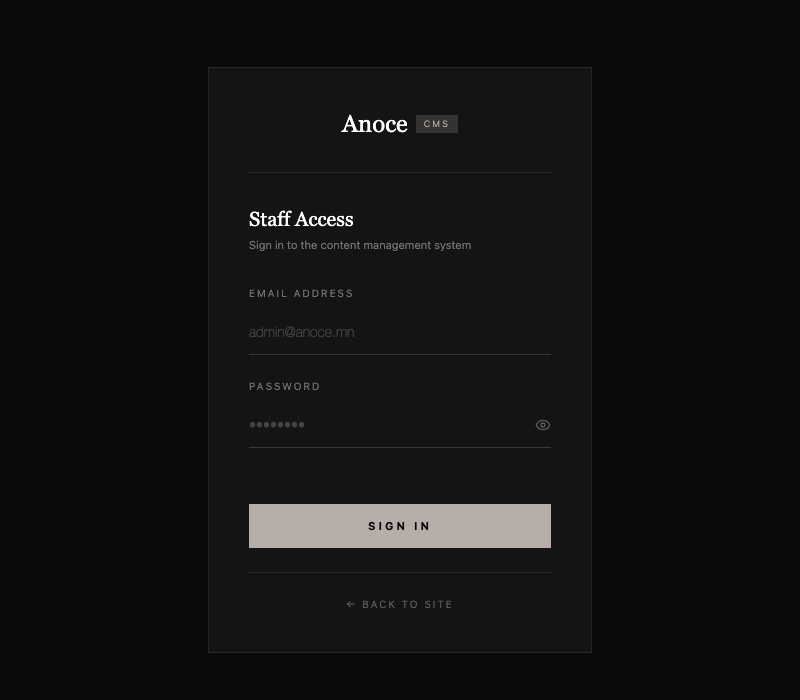
\includegraphics[width=0.72\textwidth]{Figures/screenshots/admin_login_cropped.png}
  \caption[Admin login хэрэгжилт]{Admin/редактор нэвтрэх хуудасны хэрэгжилт}
  \label{fig:impl-admin-login}
\end{figure}

\begin{longtable}{|L{0.22\textwidth}|L{0.34\textwidth}|L{0.30\textwidth}|}
  \hline
  \textbf{Үйлдэл} & \textbf{Хэрэгжилт} & \textbf{Хүлээгдэх үр дүн} \\ \hline
  Нэвтрэх & Supabase \texttt{signInWithPassword} ашиглах & Session user үүснэ \\ \hline
  Role шалгах & \texttt{profiles.role} утгыг унших & admin/editor бол CMS-д оруулна \\ \hline
  Viewer хаах & viewer role үед sign out эсвэл 403 response & Зөвшөөрөлгүй content засахгүй \\ \hline
  Protected API & \texttt{requireContentAdmin} helper ашиглах & Unauthorized үед 401, forbidden үед 403 \\ \hline
  Admin-only user management & Users page, invite API, role update API дээр admin role шалгах & Редактор хэрэглэгчийн эрх өөрчлөхгүй \\ \hline
  Account deletion & \path{/api/profile/delete} route service role ашиглан profile/bookmark/auth user устгах & Хэрэглэгч өөрийн бүртгэлээ устгана \\ \hline
  Provider key хамгаалах & Chat API server-side env ашиглах & API key browser bundle-д орохгүй \\ \hline
  \caption{Authentication ба authorization хэрэгжилт}
  \label{tab:auth-implementation}\\
\end{longtable}

Одоогийн хэрэгжилтэд уншигч, редактор, админ гурван түвшний урсгал ажиллаж байна. Редактор CMS-д контент бэлтгэж засах боломжтой боловч хэрэглэгч урих, role өөрчлөх, өөрийн role-ийг бууруулах зэрэг өндөр эрсдэлтэй үйлдэл сервер талд админ шалгалтаар хамгаалагдсан.

\section{Туршилт}
Туршилтыг functional testing, UI testing, responsive testing, security testing, AI fallback testing, build/test verification гэсэн төрлөөр төлөвлөв. Automated түвшинд repository conversion logic-ийн test байгаа бөгөөд \texttt{npm test} script-ээр ажиллана. Production build шалгахад \texttt{npm run build} ашиглана.

\begin{longtable}{|L{0.06\textwidth}|L{0.20\textwidth}|L{0.24\textwidth}|L{0.25\textwidth}|L{0.15\textwidth}|}
  \hline
  \textbf{№} & \textbf{Туршилтын нэр} & \textbf{Оролт} & \textbf{Хүлээгдэж буй үр дүн} & \textbf{Төлөв} \\ \hline
  1 & Login test & Зөв email/password & Платформд нэвтэрч session үүснэ & Шалгасан \\ \hline
  2 & Role gate test & Viewer user admin API дуудах & 403 forbidden response буцна & Шалгасан \\ \hline
  3 & Article list & \path{/api/content/articles} GET & Published articles JSON буцна & Шалгасан \\ \hline
  4 & Article create/update & Нийтлэлийн title/body/category/status & Article document нэмэгдэж, засагдана & Шалгасан \\ \hline
  5 & Collection archive & \path{/archive} нээх & Archive hero, collection/filter UI харагдана & Шалгасан \\ \hline
  6 & Search test & Keyword query & Тохирох article/collection/designer result гарна & Шалгасан \\ \hline
  7 & Review workflow & Админ нийтлэл батлах/засвар хүсэх & review note, reviewed at, status шинэчлэгдэнэ & Шалгасан \\ \hline
  8 & Admin-only role update & Редактор role API дуудах & 403 response буцна & Шалгасан \\ \hline
  9 & Account deletion & Profile delete товч дарах & profile/bookmark/auth user устгах route ажиллана & Шалгасан \\ \hline
  10 & Chatbot fallback & AI provider key байхгүй үед асуулт илгээх & Live/RAG summary эсвэл insufficient context хариу ирнэ & Шалгасан \\ \hline
  11 & Responsive test & 1440px болон mobile viewport & Text/button/card давхцахгүй & Шалгасан \\ \hline
  12 & Build/type/test & \texttt{npm run lint}, \texttt{npm test}, \texttt{npm run build} & Type check, automated test, production build алдаагүй дуусна & Шалгасан \\ \hline
  \caption{Туршилтын хүснэгт}
  \label{tab:test-cases}\\
\end{longtable}

Хөгжүүлэлтийн явцад screenshot авахдаа локал Next.js dev server ашиглаж public homepage, archive page, admin login хуудасны харагдацыг Chrome headless горимоор шалгасан. Мөн \texttt{npm run lint}, \texttt{npm test}, \texttt{npm run build} шалгалтуудыг ажиллуулж type check, repository test, production build амжилттай дууссаныг баталгаажуулсан. Security audit-ийн өндөр эрсдэлтэй асуудлыг package update-аар зассан; үлдсэн moderate түвшний PostCSS/Next зөвлөмж нь \texttt{npm audit fix --force} хийхэд Next.js-ийг хуучин major хувилбар руу бууруулах эрсдэлтэй тул тусад нь хянахаар үлдээв.

\section{Үр дүнгийн үнэлгээ}
Хөгжүүлсэн платформ нь дипломын ажлын зорилгод заасан Монголын загварын сэтгүүлийн платформын үндсэн шаардлагуудыг MVP түвшинд хангаж байна. Public талд home, archive, designers, editorial, journal, careers, press, profile, detail page, search overlay, chatbot entry point бүрдсэн. Admin талд dashboard, article/collection/designer/asset/calendar/user module, staff login, role gate, review workflow бүрдсэн. Data талд CouchDB content repository, Supabase auth/bookmark/RAG layer, монгол seed script, AI prompt/fallback бүтэц хэрэгжсэн.

\begin{longtable}{|L{0.25\textwidth}|L{0.35\textwidth}|L{0.26\textwidth}|}
  \hline
  \textbf{Үнэлэх зүйл} & \textbf{Биелсэн байдал} & \textbf{Дүгнэлт} \\ \hline
  Public fashion magazine UI & Home, editorial, archive, designer route хэрэгжсэн & Биелсэн \\ \hline
  Content management & Article, collection, designer, asset admin module хэрэгжсэн & Биелсэн \\ \hline
  Role-based access & Supabase role gate, protected admin API, admin-only users/invite/role update хэрэгжсэн & Биелсэн \\ \hline
  Database/repository & CouchDB document repository, Supabase auth/RAG layer ашигласан & Биелсэн \\ \hline
  Search/discovery & Search index API, overlay, lexical scoring хэрэгжсэн & Биелсэн, semantic search сайжруулна \\ \hline
  AI туслах & Live archive/RAG context, provider fallback бүтэцтэй & Биелсэн, dataset sync сайжруулна \\ \hline
  Responsive visual UI & Screenshot болон viewport шалгалтаар үндсэн хуудсууд харагдсан & Биелсэн \\ \hline
  \caption{Зорилго биелэлтийн үнэлгээ}
  \label{tab:result-evaluation}\\
\end{longtable}

Платформын давуу тал нь fashion magazine болон digital archive-ийн шинжийг нэгтгэсэн, зурагт контентод төвлөрсөн, CMS болон AI туслахтай, Next.js нэг codebase дотор public/admin/API-г зохион байгуулсан явдал юм. Хязгаарлалт нь production dataset бүрэн биш, Docker/CouchDB runtime орчин үргэлж асаалттай байх шаардлагатай, хайлт нь одоогоор lexical scoring төвтэй, RAG document sync manual seed script-д тулгуурлаж байгаа явдал юм.

\section{Цаашдын хөгжүүлэлт}
Цаашид платформыг дараах чиглэлээр хөгжүүлэх боломжтой:
\begin{itemize}
  \item Approval workflow дээр audit log, өөрчлөлтийн түүх, мэдэгдэл нэмэх;
  \item AI recommendation, related article/look suggestion, personalized feed хөгжүүлэх;
  \item Comment/like платформыг bookmark/follow-той уялдуулах;
  \item Semantic search, Supabase full-text/trigram/vector search нэмэх;
  \item Published content-to-RAG automatic sync хийх;
  \item Image optimization, CDN эсвэл Supabase Storage/Cloudinary migration хийх;
  \item Analytics dashboard, article performance, popular search keyword харах;
  \item Mobile app эсвэл PWA хувилбар гаргах;
  \item Fashion brand collaboration, designer submission workflow нэмэх.
\end{itemize}

\section{Бүлгийн дүгнэлт}
Дөрөвдүгээр бүлгээр Anoce/MFA платформын бодит хэрэгжилт, фронтэнд, бэкенд, өгөгдлийн сан, authentication бүтэц, screenshot, туршилт, үр дүнгийн үнэлгээ болон цаашдын хөгжүүлэлтийн чиглэлийг нэгтгэн тайлбарлав. Платформ нь одоогийн байдлаар Монголын загварын сэтгүүл-архивын MVP хувилбарыг бүрдүүлж, уншигч, редактор, админы workflow-г бодитоор дэмжих суурьтай болсон.
